%=============================================================================
%
% MULTIMAT 2024 Abstract Template
% Adapted from the 2022 template used for the Zurich meeting
%
% !!!!!!!!!!!!!!!!!!!!!!!!!!!!!!!!!!!!!!!!!!!!!!!!!!!!!!!!!!!!!!!!!!!!!!!!!!!
% !!!      ALL SUBMISSIONS MUST BE LIMITED TO 1 PAGE, NO EXCEPTIONS       !!!
% !!!    ALL SUBMISSION SHOULD CONSIST IN PDF AND EDITABLE SOURCE FILE    !!!
% !!!!!!!!!!!!!!!!!!!!!!!!!!!!!!!!!!!!!!!!!!!!!!!!!!!!!!!!!!!!!!!!!!!!!!!!!!!
%=============================================================================

%=============================================================================
%                    Formatting Options (do not modify)
%=============================================================================
\documentclass[11pt]{article}
\usepackage{geometry,times,hyperref}
\geometry{letterpaper,top=2.5cm,bottom=2.5cm,left=2.0cm,right=2.0cm}
%\usepackage[letter, margin=1in]{geometry}
\hypersetup{colorlinks=true, linkcolor=blue}
\setlength{\parindent}{0pt}
\setlength{\parskip}{5pt plus 2pt minus 1 pt}
\sloppy
\let\OLDthebibliography\thebibliography
\renewcommand\thebibliography[1]{
        \OLDthebibliography{#1}
        \setlength{\parskip}{0pt}
        \setlength{\itemsep}{3pt plus 0.3ex}
}
\newenvironment{AbstractTitle}{\begin{center} \bf \par\Large}{\par\addvspace{\bigskipamount} \end{center}}
\newcommand\email[1]{\href{mailto:{#1}}{#1}}

%=============================================================================
%                       Useful packages and commands
%=============================================================================
\usepackage{graphicx}
\usepackage{subcaption}

%=============================================================================
%                       Declarations for Front Matter
%=============================================================================
\begin{document}

\pagestyle{empty}

\begin{AbstractTitle}
  Multigroup smoothed particle radiation hydrodynamics
\end{AbstractTitle}

%
% <<< INSERT AUTHORS HERE >>> 
%
\begin{center}
\textbf{\underline{B.R. Bassett}$^\dagger$ and J.M. Owen$^\dagger$}

$^\dagger${
  Lawrence Livermore National Laboratory
             ({\tt bassett4@llnl.gov, owen8@llnl.gov}) 
          } \\
\end{center}

{\bf Keywords}: radiation hydrodynamics, multigroup diffusion, smoothed particle hydrodynamics.
To be considered for an oral presentation.

\begin{center}
\textbf{ABSTRACT}\\[1mm]
\end{center}

Smoothed particle hydrodynamics (SPH) has been coupled previously to gray radiation diffusion \cite{whitehouse}, including in our previous papers that have many similarities to this work \cite{bassett1, bassett2}. This is, to our knowledge, the first publication on multigroup radiation diffusion consistent to or coupled with SPH. We use the nonlinear elimination method in Ref. \cite{brunner} for the time update. The spatial discretization for SPH with the kernel $W_{ij}$ is performed using the same methodology as in the gray case \cite{bassett1}:

\[
\left\langle \nabla\cdot\left[D\left(x\right)\nabla\phi\left(x\right)\right]\right\rangle _{i}\approx\sum_{j}V_{j}\left(D_{i}+D_{j}\right)\left(\phi_{i}-\phi_{j}\right)\frac{x_{ij}^{\alpha}}{x_{ij}^{\beta}x_{ij}^{\beta}}\partial_{x_{i}}^{\alpha}W_{ij}.
\]

For reproducing kernels (RK) $U_{ij}$, which guarantee that the kernels reproduce a chosen order of polynomials exactly, the diffusion operator is 

\[
\left\langle \nabla\cdot\left[D\left(x\right)\nabla\phi\left(x\right)\right]\right\rangle _{i}\approx\frac{1}{2}\sum_{j}V_{j}\left(D_{i}+D_{j}\right)\left(\phi_{j}-\phi_{i}\right)\nabla^{2}U_{ij}.
\]

For a complete derivation of this derivative, see Ref. \cite{bassett3}. The SPH derivatives are generally preferred for shock problems, where the less-reactive diffusion operator provides some smoothing. The RK derivatives function well in smooth problems but struggle in the presence of shocks. 

Figures \ref{fig:sph-conv} to \ref{fig:sph-conv-2d} show convergence of the material and radiation energies for a sinusoidal manufactured solution. The SPH results are consistent with the expected second-order convergence, while the RK results with quadratic corrections are consistent with the expected third-order convergence. The presentation will further explore equilibration and time-dependent results. 

\begin{figure}[htbp]
\centering
\begin{subfigure}{0.32\textwidth}
  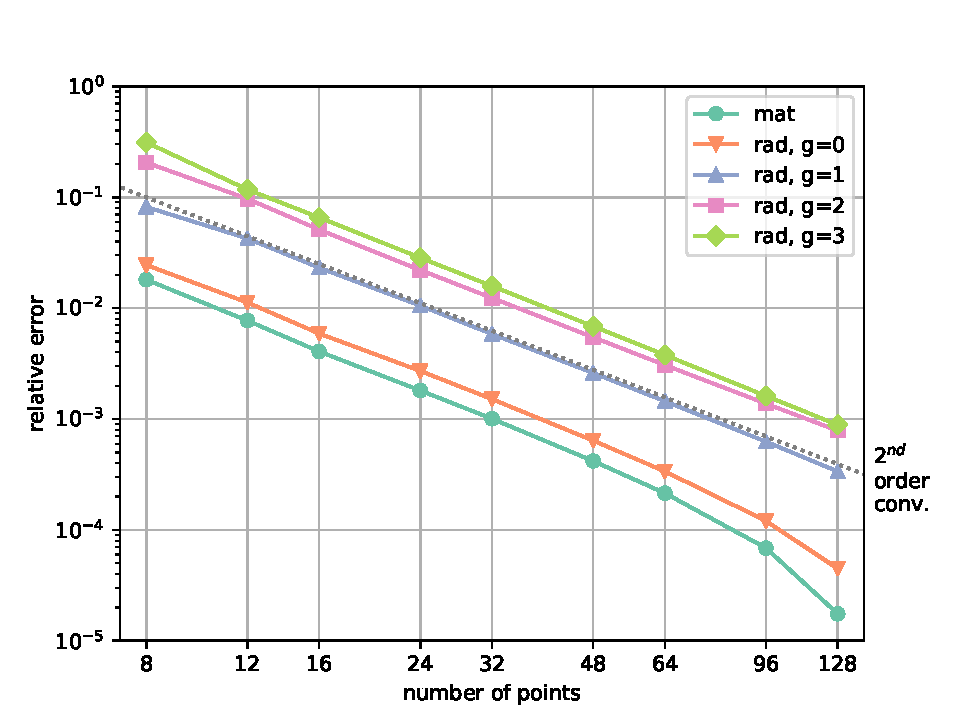
\includegraphics[width=\linewidth]{../figs/ManufacturedConvergence1d}
  \caption{SPH diffusion, 1D}
  \label{fig:sph-conv}
\end{subfigure}
\hfill
\begin{subfigure}{0.32\textwidth}
  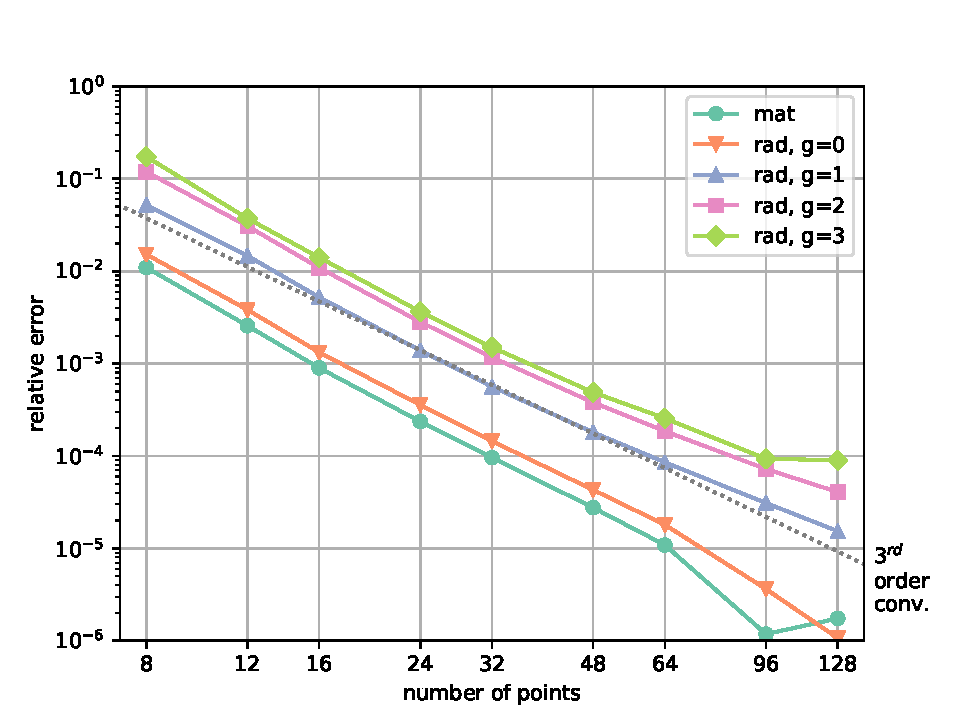
\includegraphics[width=\linewidth]{../figs/ManufacturedConvergenceRK1d}
  \caption{RK diffusion, 1D}
  \label{fig:rk-conv}
\end{subfigure}
\hfill
\begin{subfigure}{0.32\textwidth}
  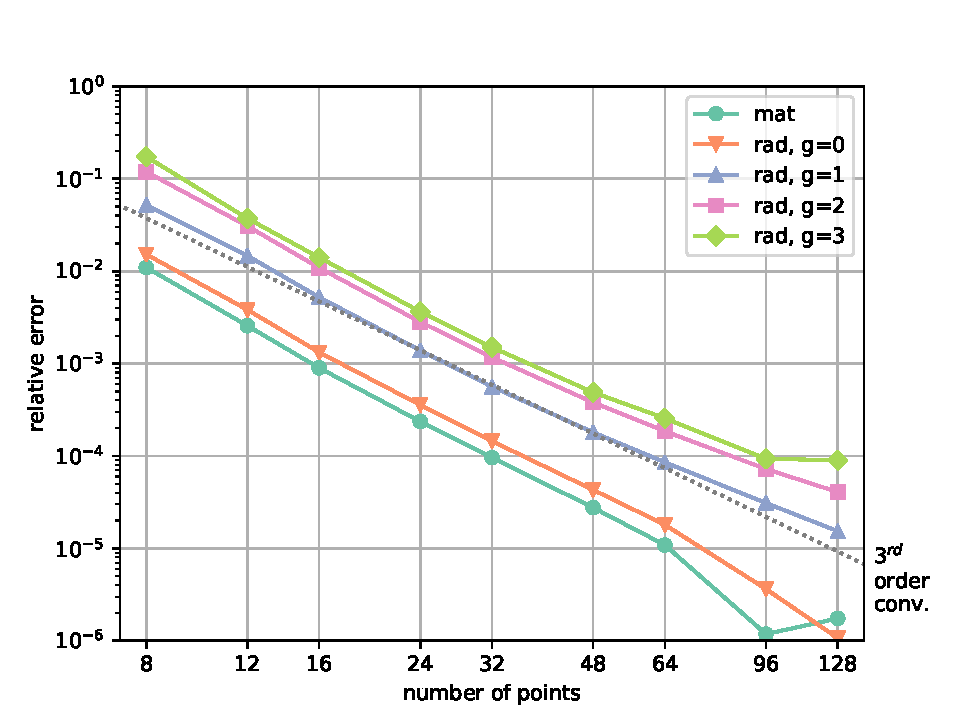
\includegraphics[width=\linewidth]{../figs/ManufacturedConvergenceRK1d}
  \caption{SPH diffusion, 2D}
  \label{fig:sph-conv-2d}
\end{subfigure}
\caption{Convergence plots for multigroup diffusion}
\end{figure}

\begin{thebibliography}{10}
\bibitem{whitehouse} S.C. Whitehouse, M.R. Bate and J.J. Monaghan,
  ``A faster algorithm for smoothed particle hydrodynamics with radiative transfer in the flux-limited diffusion approximation''
  \textit{Monthly Notices of the Royal Astronomical Society}, 364(4), pp.~1367--1377, 2005.
\bibitem{bassett1} B.R. Bassett, J.M. Owen and T.A. Brunner,
  ``Efficient smoothed particle radiation hydrodynamics I: Thermal radiative transfer''
  \textit{Journal of Computational Physics}, 429, pp.~109996, 2021.
\bibitem{bassett2} B.R. Bassett, J.M. Owen and T.A. Brunner,
  ``Efficient smoothed particle radiation hydrodynamics II: Radiation hydrodynamics''
  \textit{Journal of Computational Physics}, 429, pp.~109994, 2021.
\bibitem{brunner} T.A. Brunner, T.S. Haut and P.F. Nowak,
  ``Nonlinear Elimination Applied to Radiation Diffusion''
  \textit{Nuclear Science and Engineering}, pp.~1--13, 2020.
\bibitem{bassett3} B.R. Bassett and J.M. Owen,
  ``CRKSPH-compatible discretization of the SUPG and SAAF transport equations''
  \textit{Nuclear Science and Engineering}, pp.~1--13, 2020.
\end{thebibliography}

This work was performed under the auspices of the U.S. Department of Energy by Lawrence Livermore National Laboratory under Contract DE-AC52-07NA27344. LLNL-ABS-863622.

\end{document}
